\clearpage

\renewcommand{\thesection}{\Alph{section}} % Change numbering to letters
\setcounter{section}{0} % Reset section counter
\setcounter{table}{0}
\setcounter{figure}{0}
\maketitlesupplementary


\section{Model Details}
\subsection{Implementation Details}
For the vision backbone, we use Swin Transformer that is pre-trained on ImageNet. For the text encoder, we use the text encoder from the open-sourced CLIP\footnote{\url{https://github.com/openai/CLIP}}. During Hungarian matching, we only use classification loss, box L1 loss, and GIOU loss. The loss weights are 2.0, 5.0, and 2.0, respectively. For the final loss, we use classification loss, box L1 loss, GIOU loss, and constrastive loss, and set the weights to be 1.0, 5.0, 2.0, and 1.0, respectively. Following DINO, we use contrastive denoising training (CDN) to stabilize training and accelerate convergence.

We use automatic mixed precision for training. For the Swin Transformer tiny model, the training is performed on 16 NVIDIA A100 GPUs with a total batch size of 128. For the Swin Transformer large model, the training is performed on 32 NVIDIA A100 GPUs with a total batch size of 64.

\section{Data Engine Details}
\subsection{Text Prompt Data Engine}
To collect region-text pairs from caption datasets LAION400M and Conceptual Captions, We first use CLIP to compute the CLIP score for each image and its caption and retain only pairs of image descriptions with similarity greater than 0.8. Next, we use spaCy to extract the noun phrases in each caption and then use these nouns to prompt the GroundingDINO model to get the box regions corresponding to these noun phrases in the image. Finally, we will compute the CLIP score for each box region and its corresponding noun phrases once more, and keep only the pairs with similarity greater than 0.8.

\subsection{Image Prompt Data Engine}
\begin{figure}[h]
\centering

\includegraphics[width=\linewidth]{images/data_engine.pdf}\vspace{-1mm}
\caption{Workflow of the proposed image prompt data engine.}
\label{fig:data_engine}
\vspace{-1mm}
\end{figure}


We show the overview of the proposed data engine in Fig. \ref{fig:data_engine} and some examples in DetSA-1B in Fig. \ref{fig:detsa_1b}.



\begin{figure*}[t]
\centering
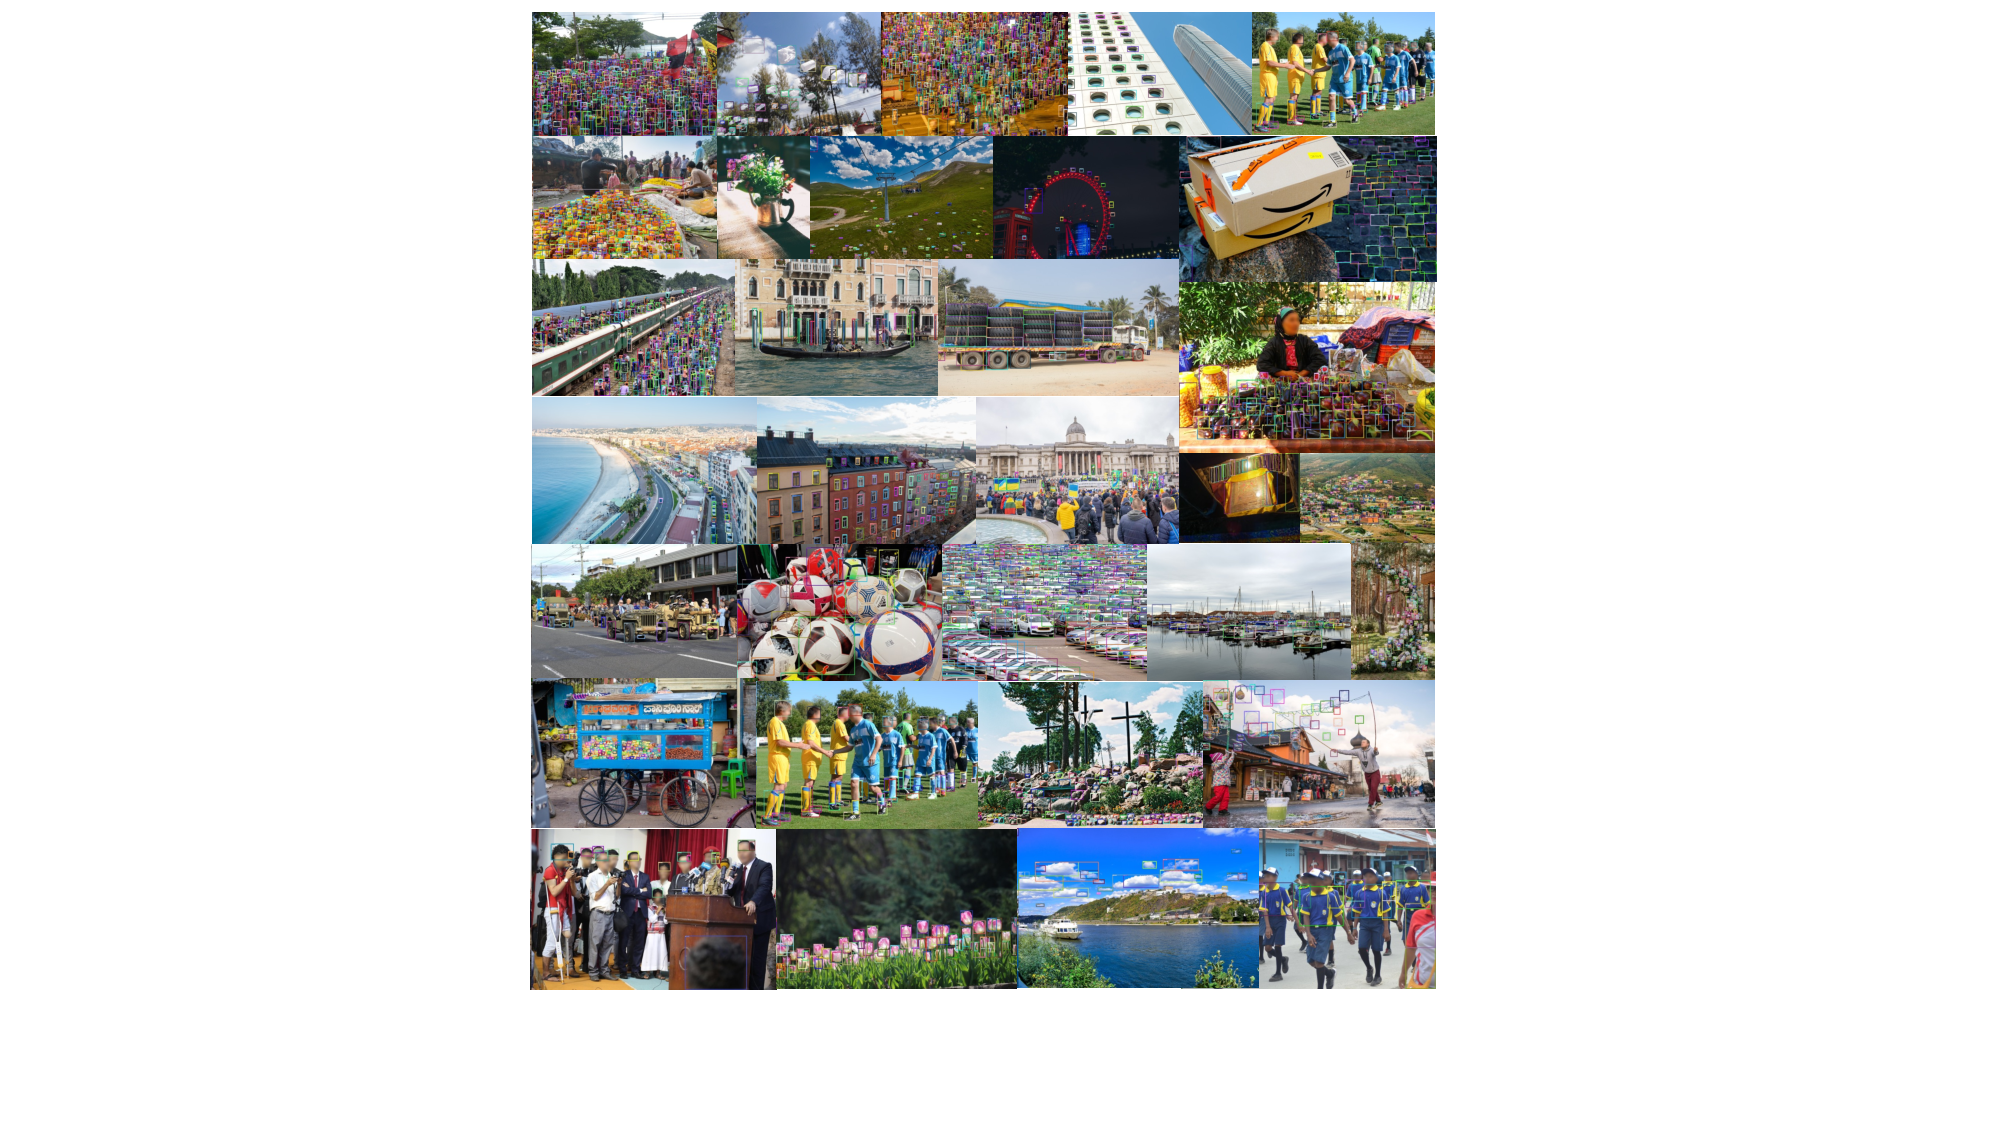
\includegraphics[width=\linewidth]{images/detsa_1b.pdf}\vspace{-1mm}
\caption{Examples in DetSA-1B.}
\label{fig:detsa_1b}
\vspace{-1mm}
\end{figure*}

\subsection{Data Statistics}


\begin{table}[]
  \centering
  \resizebox{\columnwidth}{!}{%
    \begin{tabular}{c|c|c}
\hline
Data Type                    & Dataset             & \# Images \\ \hline
\multirow{3}{*}{Text prompt} & Conceptual Captions & 1,840,473 \\
                             & LAION400M           & 1,202,245 \\
                             & Bamboo              & 1,109,856 \\ \hline
Visual Prompt                & SA-1B               & 653,285   \\ \hline
\end{tabular}}
\caption{Data statistics of data collected from text prompt and visual prompt engines.}
\label{tab:data_statistics}
\end{table}


We list the amount of data collected from the two data engines in Tab. \ref{tab:data_engine}.
\begin{figure*}[ht]
\centering
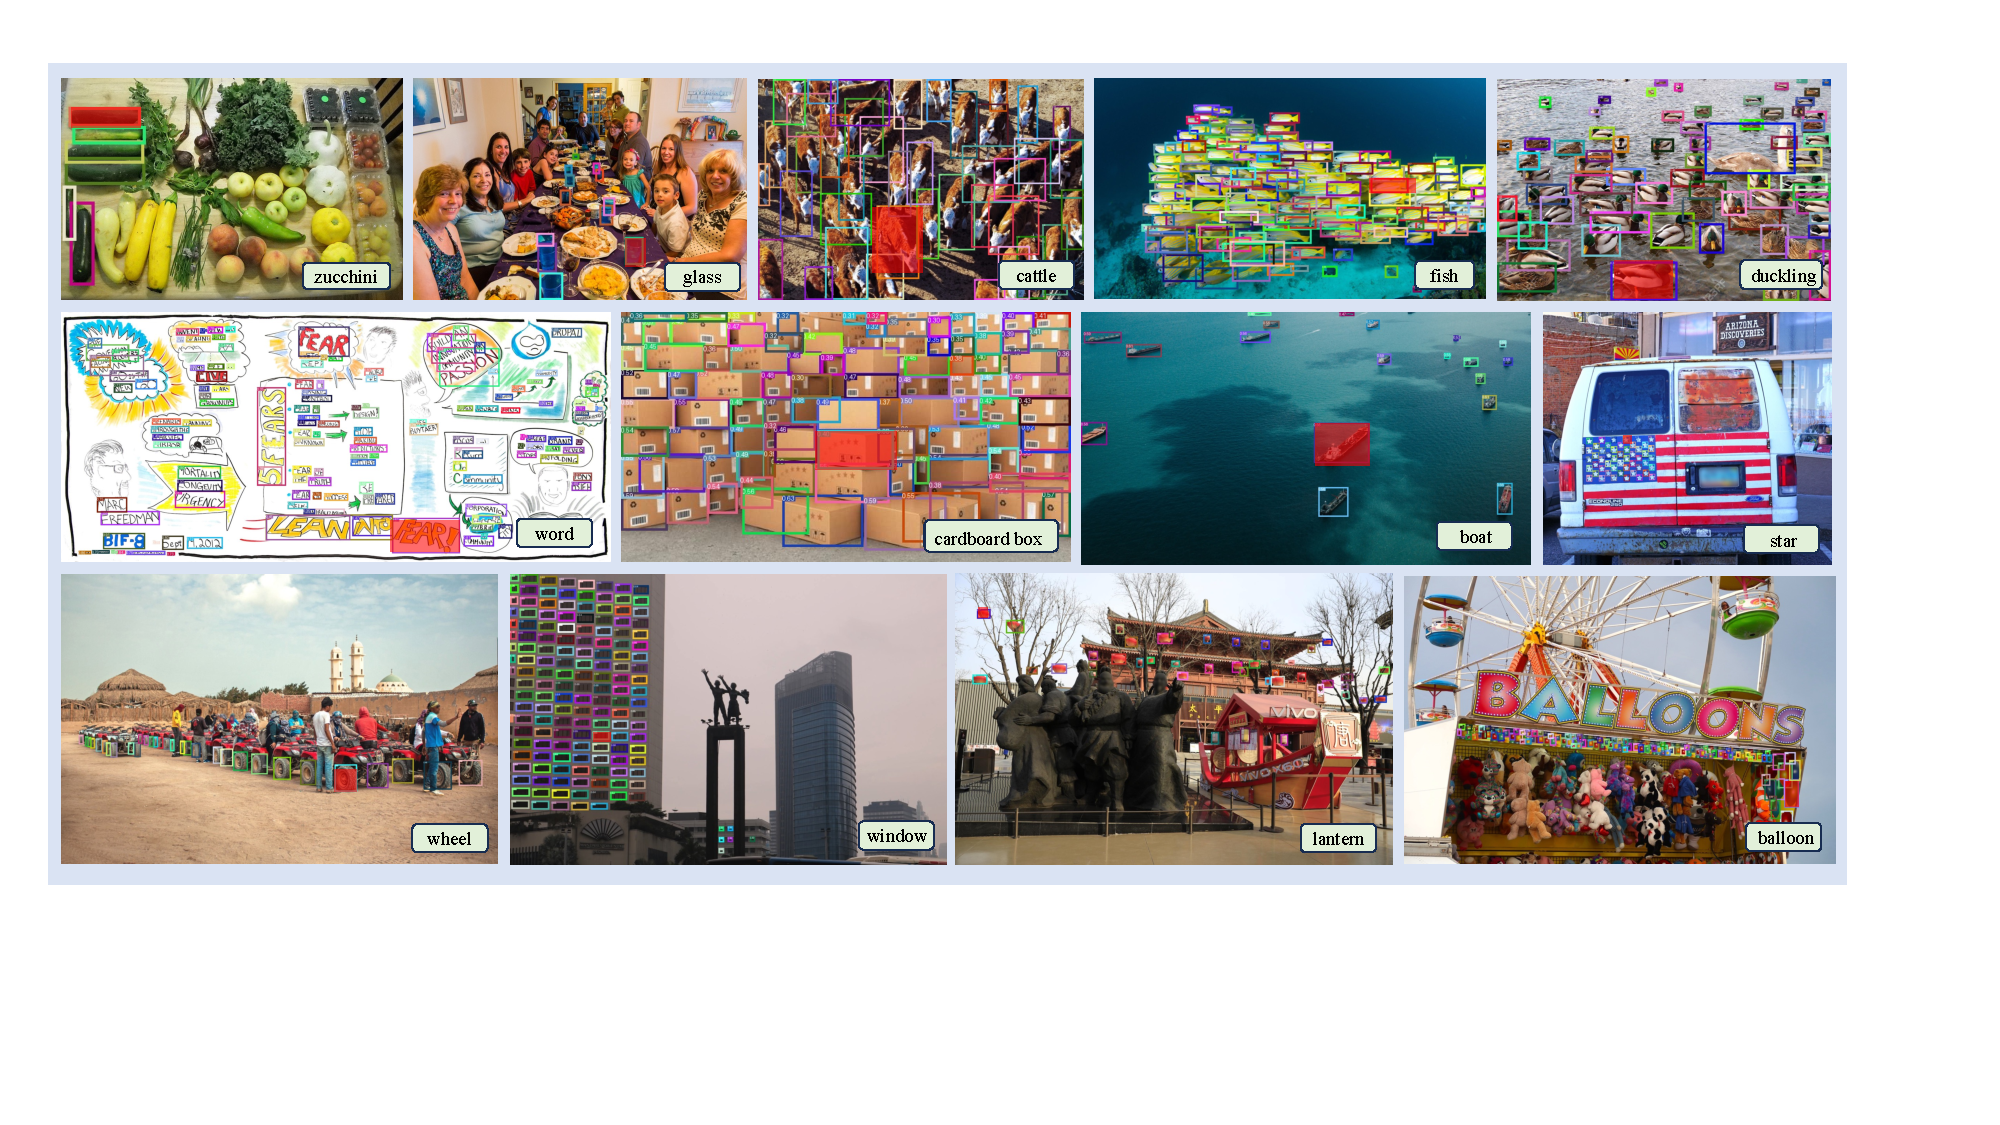
\includegraphics[width=\linewidth]{images/sup_region_classify.pdf}\vspace{-1mm}
\caption{Visualization results of region classification workflow. We use a dictionary of 2560 classes to classify the visual prompts. The classification result is shown at the bottom right for each image.}
\label{fig:region_class}
\vspace{-1mm}
\end{figure*}


\section{Advanced Capabilities for T-Rex2}
\subsection{Region Classification}
\label{sec:Region}
Beyond the aforementioned three inference workflows, \ourmodel{} also supports the capability of region classification. The contrastive alignment between text prompts and visual prompts also unlocks the capability to classify regions for visual prompts. Much like the zero-shot classification approach of CLIP, we can assign category labels to visual prompts by measuring the similarity between visual prompts and pre-computed text prompts:
\begin{equation}
\operatorname{Label} = \operatorname{argmax}j \left(\frac{\exp(V \cdot t_j)}{\sum_{l=1}^K \exp(V \cdot t_l)}\right)
\end{equation}
We can use predefined category names to pre-compute the text embeddings which enable us to identify arbitrary objects through visual prompting. 

We show the zero-shot region classification results on COCO and LVIS in Tab. \ref{tab:region_classification}. We use each GT box as the visual prompt and compute the similarity with all the category names in that dataset. Compared to CLIP, \ourmodel{} possesses stronger region classification capability. We show some visualization results in Fig. \ref{fig:region_class}.


\begin{table}[]
  \centering
  \resizebox{\columnwidth}{!}{%
    \begin{tabular}{cc|cc|cc}
\hline
\multirow{2}{*}{Method} & \multirow{2}{*}{Backbone} & \multicolumn{2}{c|}{\begin{tabular}[c]{@{}c@{}}COCO-Val\\ Zero-Shot\end{tabular}} & \multicolumn{2}{c}{\begin{tabular}[c]{@{}c@{}}LVIS-Val\\ Zero-Shot\end{tabular}} \\ \cline{3-6} 
                        &                           & Acc@Top1                                & Acc@Top5                                & Acc@Top1                                & Acc@Top5                               \\ \hline
CLIP                    & ViT-B                     & 37.6                                    & 60.1                                    & 9.0                                     & 20.0                                   \\ \hline
T-Rex2                   & Swin-T                    & 72.6                                    & 89.4                                    & 40.8                                    & 67.5                                   \\
T-Rex2                   & Swin-L                    & \textbf{82.2}                                    & \textbf{93.9}                                    & \textbf{49.8}                           & \textbf{76.9}                          \\ \hline
\end{tabular}}
\caption{Zero-shot region classification results. For each dataset, we use its full categories as the classification target and calculate the Top1 and Top5 classification accuracy. For CLIP, we crop the region out for classification.}
\label{tab:region_classification}
\end{table}


\subsection{Open-set Video Object Detection}
\ourmodel{} can also be used for open-set video object detection. Given a video, we can extract any $N$ frames, customize a generic visual embedding for a certain object by using T-Rex2's generic visual prompt workflow, and then use this embedding to detect all frames in the video. We also show some visualization results in Fig. \ref{fig:video_demo}. Despite not being trained on video data, T-Rex2 can also detect objects in videos well. 

\begin{figure*}[ht]
\centering
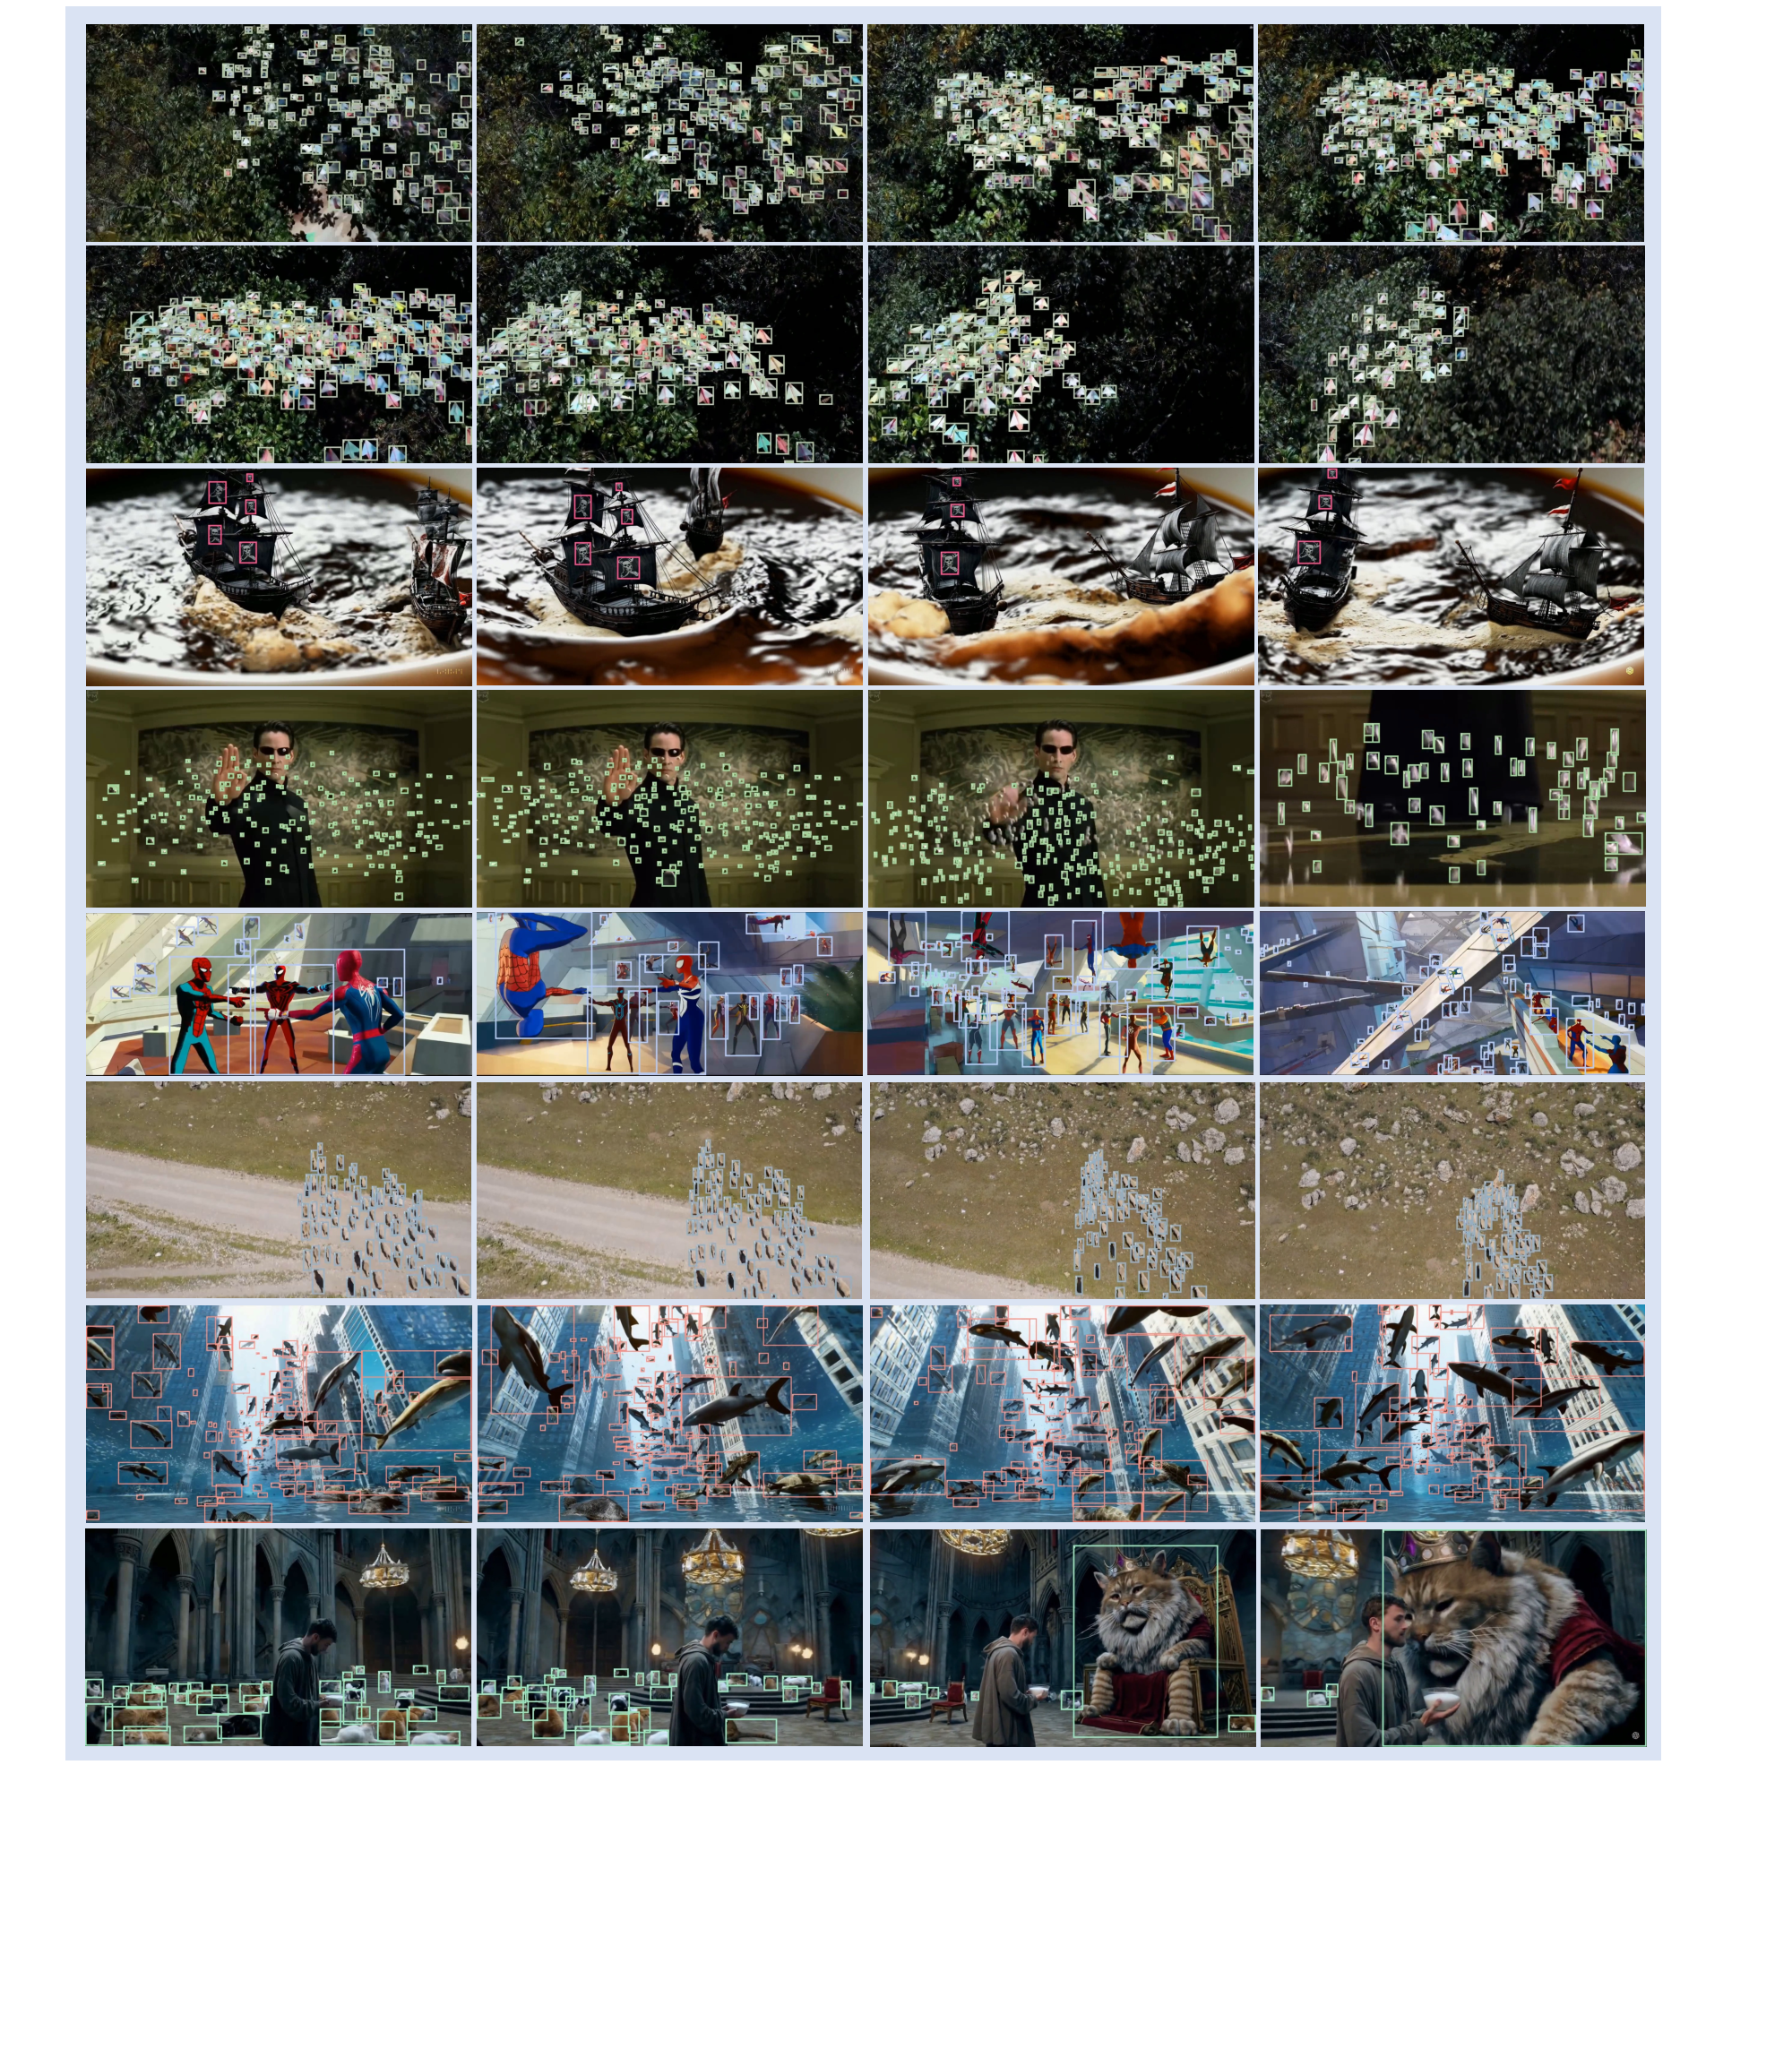
\includegraphics[width=0.8\linewidth]{images/video_demo.pdf}\vspace{-1mm}
\caption{\ourmodel{} on zero-shot video object detection task. We randomly sample 4 frames from a given video and customize a generic visual embedding for an object through the generic visual prompt workflow of \ourmodel{}. This visual embedding will be used for inference for all video frames.}
\label{fig:video_demo}
\vspace{-1mm}
\end{figure*}

\section{More Experiment Details}
\subsection{Details on Object Counting Task}
We evaluate \ourmodel{} on the object counting task to show its interactive object detection capability. Specifically, we are focusing on the few-shot object counting task. In this task, each image will be provided with three exemplar boxes on the current image to indicate the target object and require the output of the number of the target object.

\textbf{Settings.} We conduct evaluations on the commonly used counting dataset FSC147 and the more challenging dataset FSCD-LVIS. FSC147 comprises 147 categories of objects and 1190 images in the test set and FSCD-LVIS comprises 377 categories and 1014 images in the test set. Both
two datasets provide three bounding boxes of exemplar objects for each image, which we will use as the visual prompt for T-Rex2.

\textbf{Metric.} We adopt the Mean Average Error (MAE) metric, a widely employed standard in object counting. The mathematical expression is as follows:
\begin{equation}
    \mathrm{MAE}=\frac{1}{J} \sum_{j=1}^J\left|c_j^*-c_j\right|
\end{equation}
We report MAE on the FSC147 dataset as it doesn't provide ground truth boxes on test set images, and report AP on the FSCD-LVIS dataset as it provides ground truth boxes. We show some prediction results of T-Rex2 on the FSC147 and FSCD datasets in Fig. \ref{fig:counting_vis}.

\subsection{Visualization Comparison with T-Rex}
In Fig. \ref{fig:trex12}, we compare the detection results for T-Rex and \ourmodel{}. In interactive visual prompt detection mode, both models exhibit comparable performance in single-object scenes (where there is no interference from other objects in the image). For multi-object scenarios, T-Rex is more prone to false detections, whereas \ourmodel{} exhibits fewer false detections, indicating a better distinction between objects. This improvement is attributed to the joint training with text and visual prompts. For generic visual prompt detection mode, \ourmodel{} also shows more advantages.


\begin{figure*}[t]
\centering
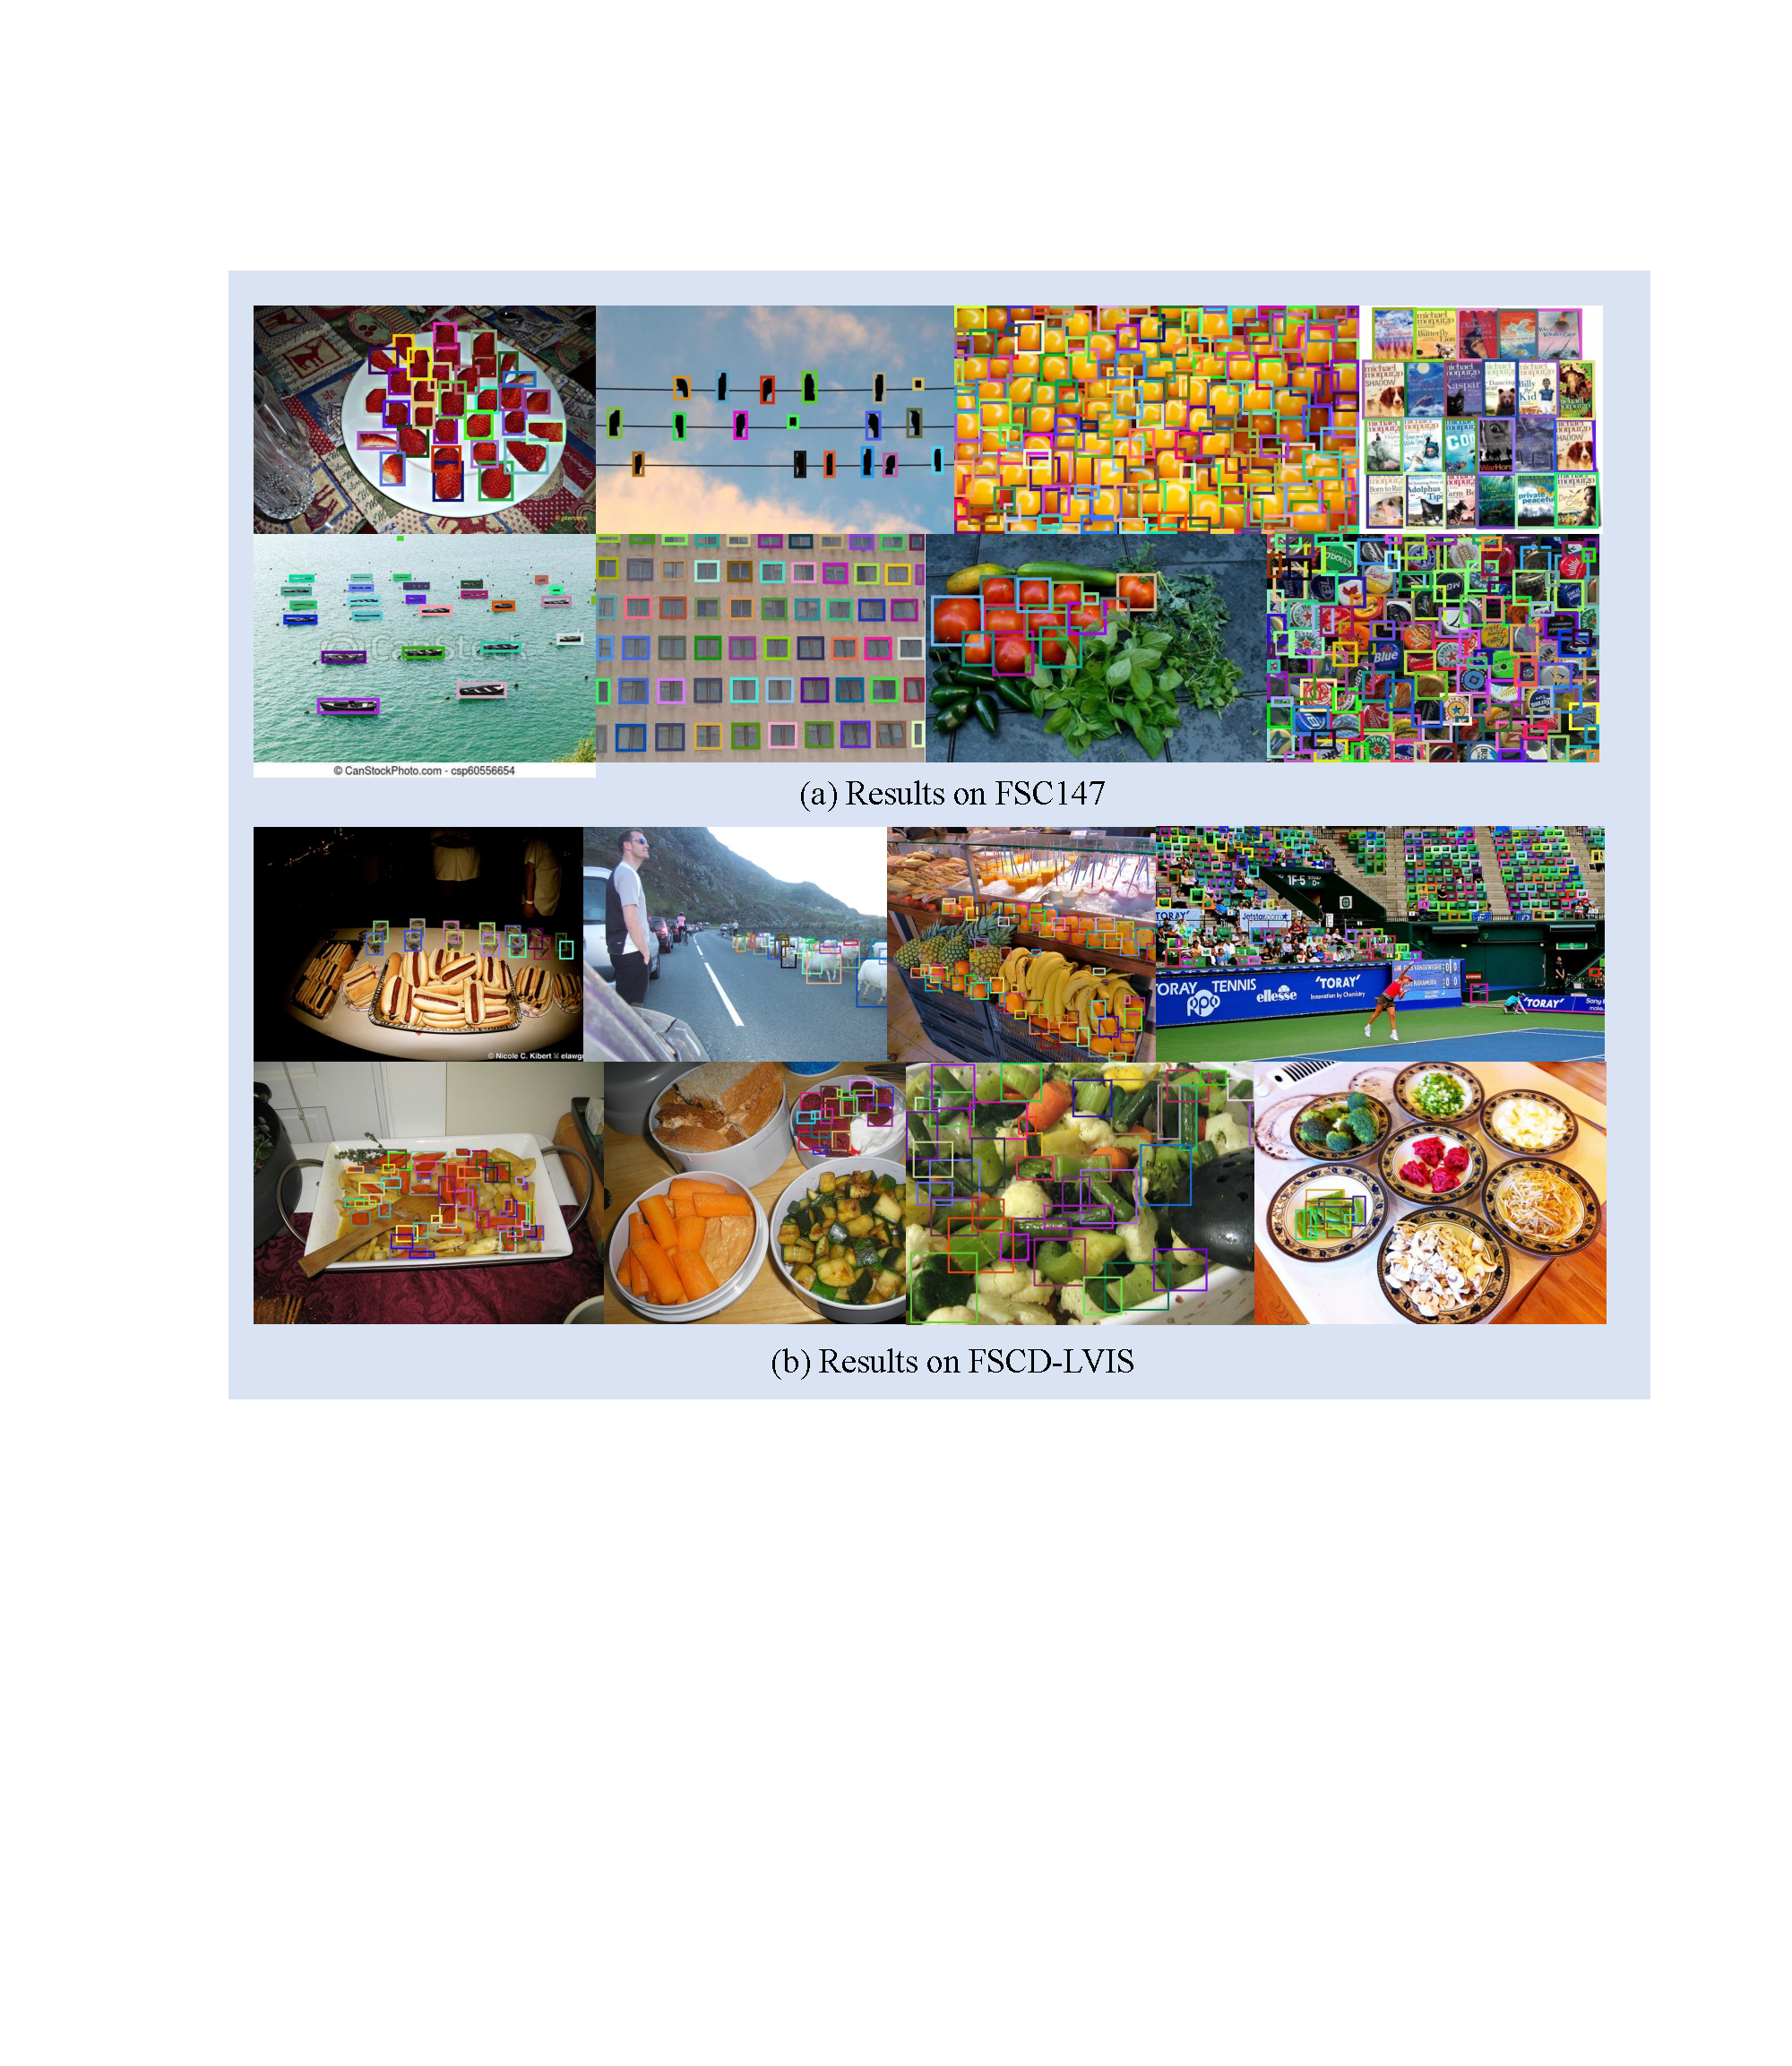
\includegraphics[width=\linewidth]{images/counting_vis.pdf}\vspace{-1mm}
\caption{The prediction results of \ourmodel{} on the FSC147 and FSCD-LVIS datasets, respectively.}
\label{fig:counting_vis}
\vspace{-1mm}
\end{figure*}

\begin{figure*}[t]
\centering
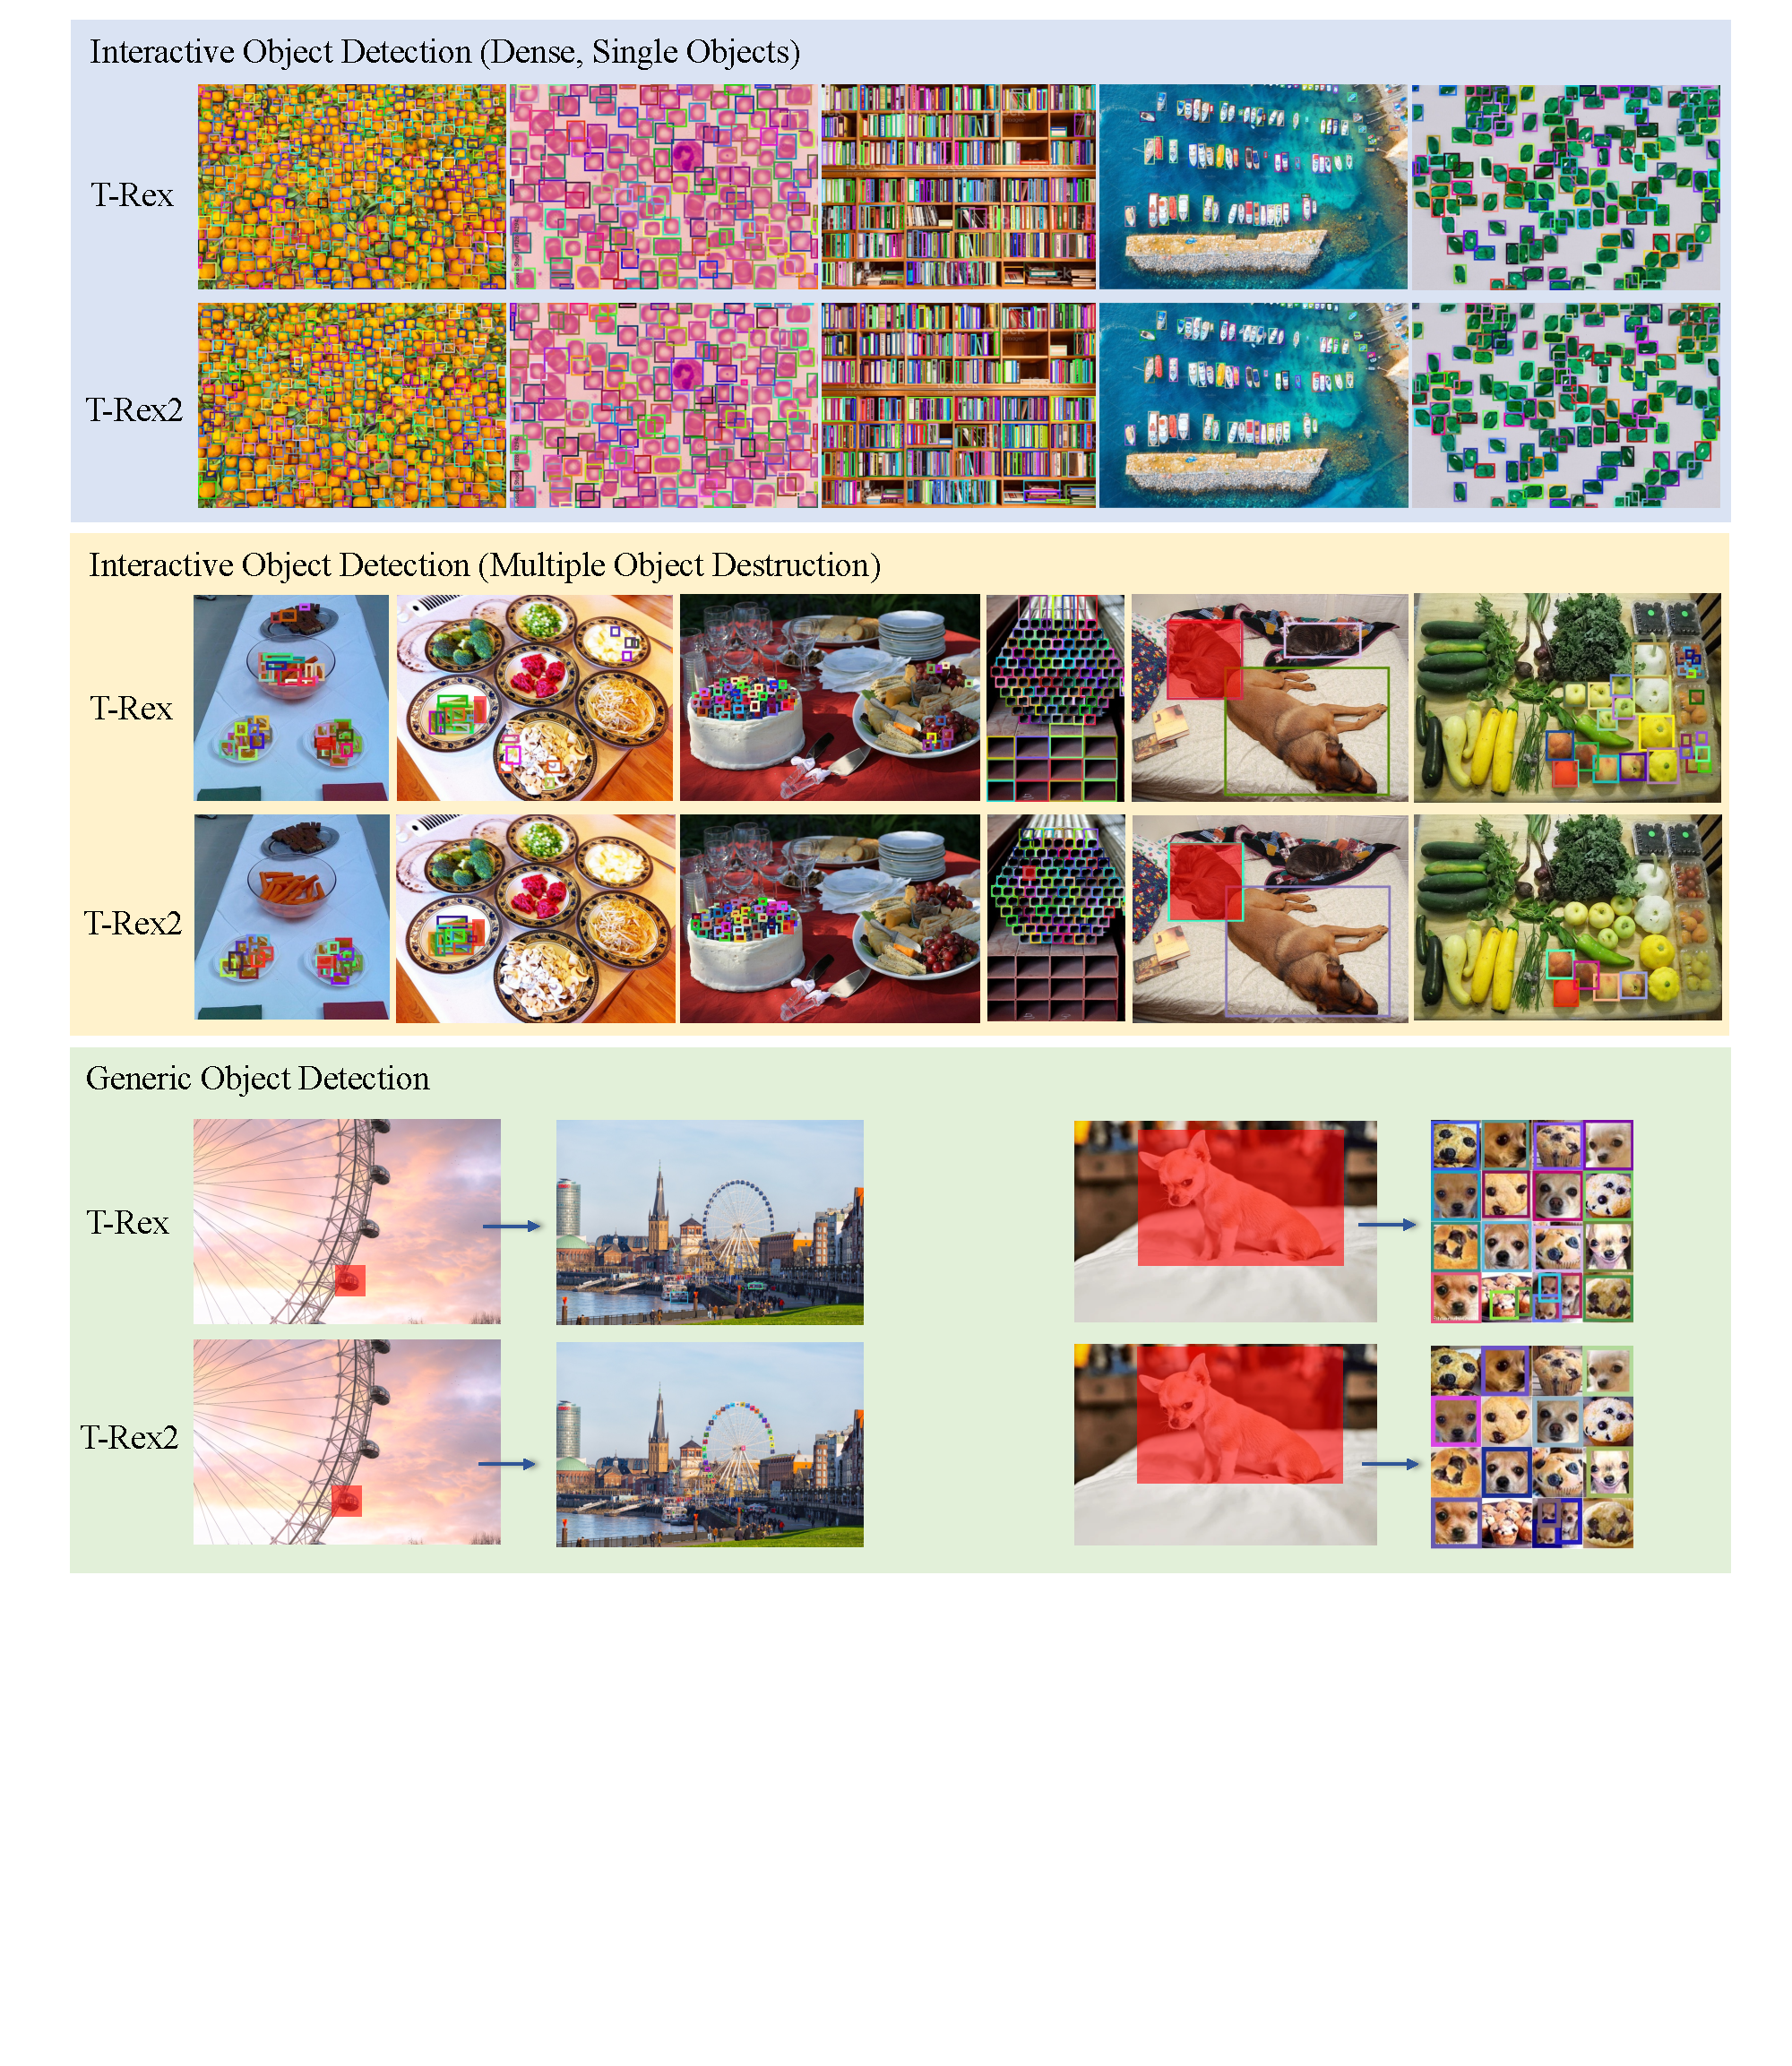
\includegraphics[width=\linewidth]{images/compare_trex.pdf}\vspace{-1mm}
\caption{Visualization comparison between T-Rex and \ourmodel{}.}
\label{fig:trex12}
\vspace{-1mm}
\end{figure*}
